\documentclass[a4paper,UTF8]{article}
\usepackage{ctex}
\usepackage{graphicx}
\usepackage{geometry}
\usepackage{float}
\geometry{left=2.54cm,right=2.54cm,top=2.54cm,bottom=2.54cm}
%opening
\title{ 计算机网络项目报告\\[0.5em]E-mail and GPG based \\ Secured Instant Message Application}
\author{11510035\quad 彭一明\\11510050\quad 王戈扬 \\ 11510352\quad 李子强\\11510086\quad 毛玉莲}

\begin{document}

\maketitle

\begin{abstract}
在项目中,我们利用如今广泛使用的邮件系统为基础,使用非对称加密算法实现了端对端加密的准即时通信。我们在Spring Boot框架下配置数据源和通过Jdbc Template编写数据访问,搭建了公钥的服务器。新用户使用邮箱和密码创建用户账号,应用根据RSA算法生成一对公钥和私钥,然后客户端将公钥与用户的邮箱账号一起上传服务器,私钥存在本地。客户端从服务器获取消息接收人的公钥,将用户的消息加密,并通过邮件发送到消息接收人的邮箱,消息接收人的客户端从邮件服务器中取出新邮件并用本地私钥解密,显示新信息在应用界面上。
\end{abstract}
\section{实现方法}
\subsection{设计模式 - 观察者模式}
	定义对象间的一种一对多的依赖关系,当一个对象的状态发生改变时,所有依赖于它的对象都得到通知并被自动更新。
	本项目中,实现后台不断进行新邮件轮询。如出现新邮件调用前端函数进行自动更新。这样降低了,前后端的耦合度,并建立一套触发机制。
\subsection{依赖库、平台}
\begin{itemize}
	\item 程序语言:Python 3
	\item 支持平台:Windows,Linux
	\item 加密服务器\\
	Spring Boot框架下配置数据源,通过Jdbc Template编写数据访问Mysql数据库
	\item GUI\\
	使用PyQt5实现GUI
	\begin{itemize}
		\item 登陆界面\\
		登陆界面提供用户邮箱、密码两个输入框,设置和登录两个按钮。用户可以点击设置按钮,设置邮件服务提供商,邮件服务器和端口号,还有修改锁屏密码。
		\begin{figure}[H]
			\centering
			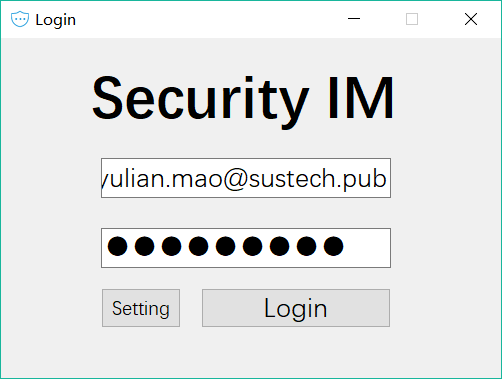
\includegraphics[width=0.5\textwidth]{UI2.png} 
			\caption{登录窗口}
			\label{fig:Log_in}
		\end{figure}
		\item 消息界面 
		左侧栏是会话列表,右上是历史聊天消息浏览框,右下是聊天输入框,还有发送按钮,图片、附件发送按钮。
		\\右键左侧会话列表,可以快捷添加成员。
		\\双击会话,弹出当前会话详情,显示群组成员。右键成员可以屏蔽其发出的消息。
	\end{itemize}
\item 加密解密\\
 使用Python的第三方库:
 \begin{itemize}
 	\item rsa\\
 	生成一对公钥和私钥
 	\item Cipher,algorithms,default\_backend\\
 	加密解密消息
 	\item base64\\
 	解决编码问题
 
 \end{itemize}
\end{itemize}

\section{软件功能}
\begin{itemize}
	\item 用户登陆\\
	用户通过使用邮箱和邮箱密码登陆,系统会使用RSA算法生成一对公钥和私钥匹配给用户,并在本地新建一个用户数据文件夹,用来存储用户的私钥和收到的文件。
	\item 收发消息(单人 / 群组)\\
	用户在选定会话(单人会话或多人会话)后,在消息框中输入待发送的消息,消息支持\textbf{中英文},点击发送。系统会在服务器上取回相应的公钥,加密后发送到联系人的邮箱。\\
	系统定时检查邮箱中是否有新的邮件,并拉取新邮件,使用本地私钥解密后在用户界面显示。
	\item 收发图片、附件\\
	与收发消息的机理相同,附件会保存在用户数据文件夹。
	\item 密钥功能\\
	实现公钥私钥的添加、更新、删除。
	\item 联系人管理\\
	用户可以给联系人进行备注,可以新建群,系统会给每个联系人,每个群组分配一个UID,发送消息时,邮件的主题为UID,系统通过UID来识别不同的联系人,联系群组。同时,用户可以添加、删除联系人,群组。
\end{itemize}
\begin{figure}[H]
	\centering
	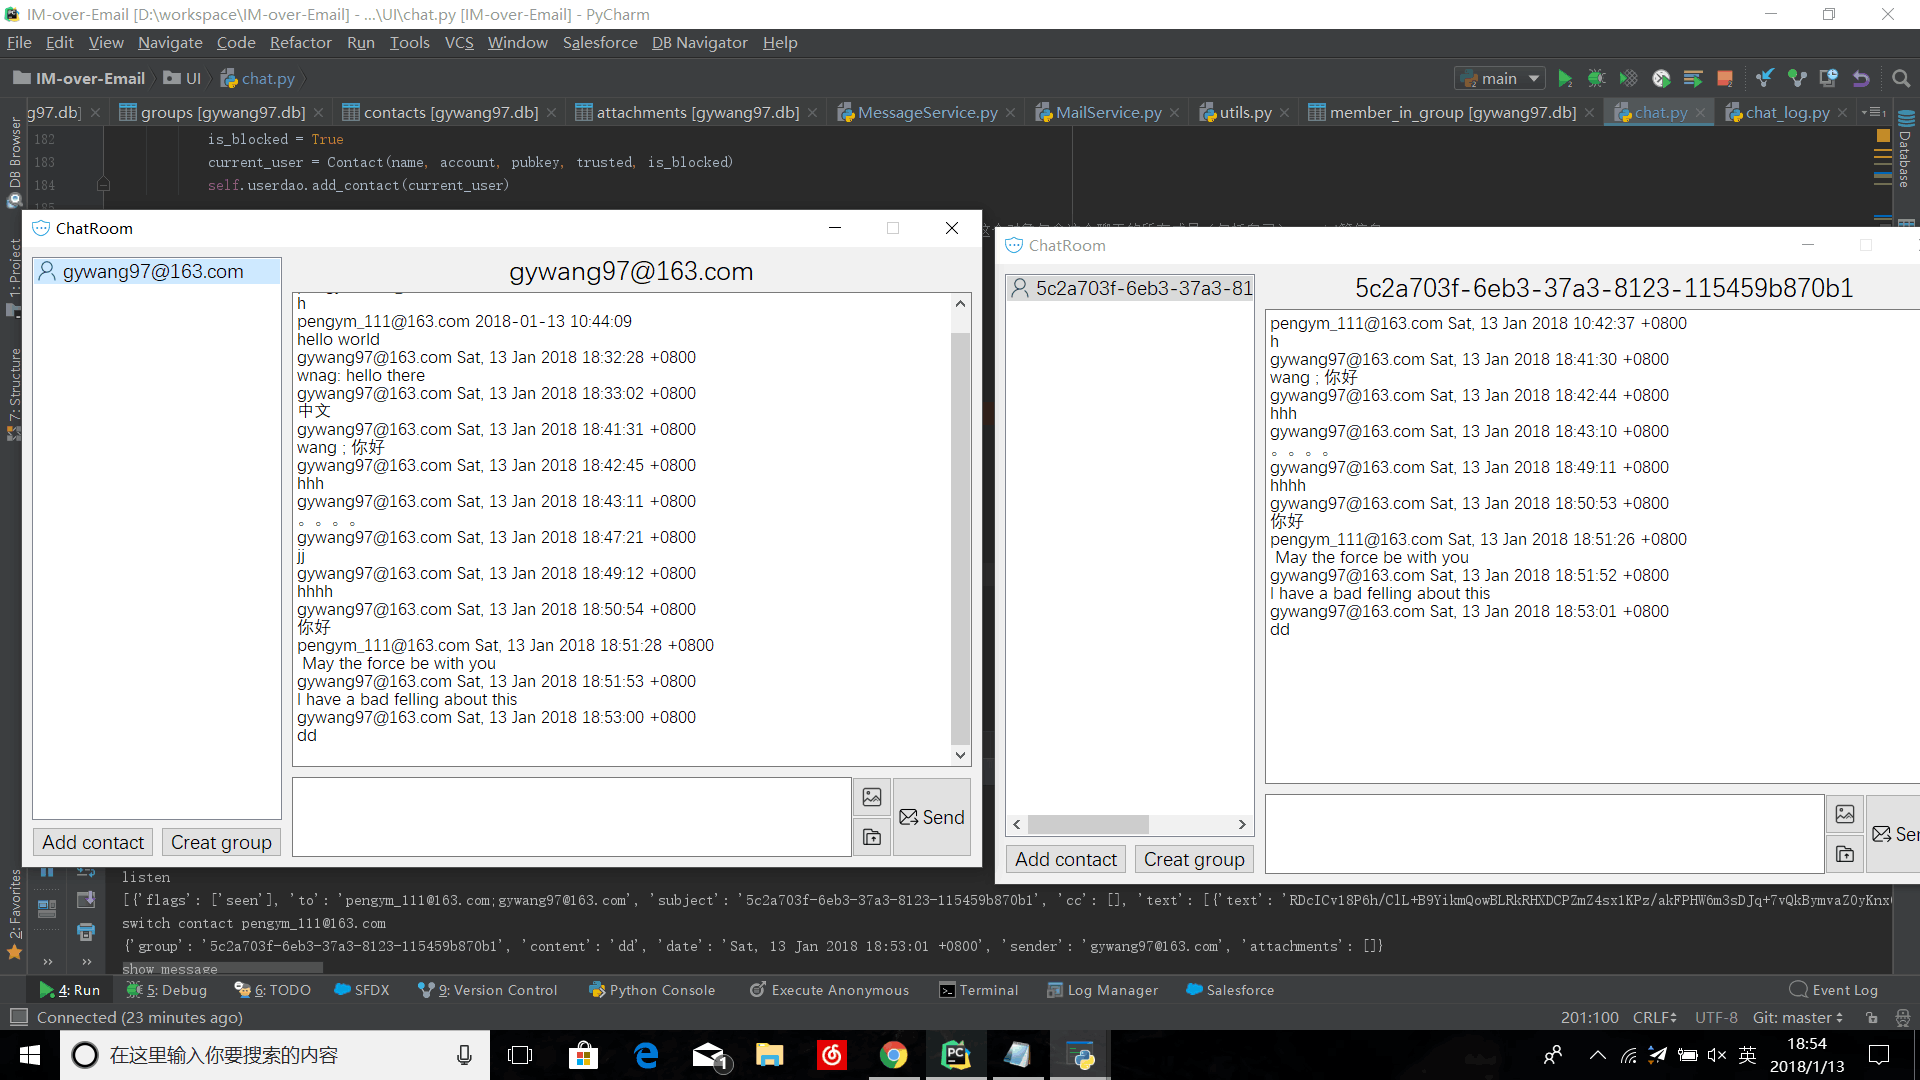
\includegraphics[width=\textwidth]{UI1.png} 
	\caption{聊天窗口}
	\label{fig:Chatting_win}
\end{figure}

\section{项目细节}
\subsection{项目分工}
\begin{itemize}
	\item 彭一明
	\\IMAP,SMTP协议读写邮件,数据库持久化操作,公钥服务器的配置和部署。
	\item 王戈扬
	\\消息加密,解密的实现,与公钥服务器的对接。

	\item 李子强
	\\软件UI设计和实现。

	\item 毛玉莲
	\\GnuPG加密解密,将公钥上传服务器。
\end{itemize}
\subsection{项目感想}

\subsubsection{彭一明}
在本次项目中我主要做了以下的工作:
\begin{enumerate}
\item 使用Python的imap和smtp库进行邮件的收发工作。这是本次项目最底层的代码,所以我尽可能的实现了邮件收发的所有功能:
	\begin{enumerate}
	\item 给多个用户发送带多个附件的功能
	\item 接收带多个附件的功能
	\item 解决了邮件中棘手的编码解码问题
	\end{enumerate}
	我详细的测试了这些功能,这些可靠的函数为后面的开发带来了极大地方便。

\item 数据库的设计和实现
本次项目采用了类似于QQ的架构,为每个用户创建单独的文件夹,在文件夹内存储用户加密过的私钥、用户数据库、接收到的附件。
所以整个项目的数据库设计分为两个部分:
	\begin{enumerate}
		\item 主数据库,用于存储多用户的基本信息
		\item 用户数据库,用于存储聊天信息,联系人信息,黑名单信息等用户信息。
	\end{enumerate}
随着项目的进行,我也经常根据小组开发的需求对数据库的架构进行迭代升级,保证用户数据稳定可靠地存储到数据库中。
	\item Model层的实现
	\\我负责提供上层函数和数据库交互的API
	\begin{enumerate}
		\item 主数据库API,新增用户,验证用户信息等功能。
		\item 用户数据库API, 联系人,群组,消息,附件, 黑名单等的CRUD(Create, Retrieve, Update, Delete)操作。
	\end{enumerate}
这些API是实现用户逻辑的核心。这些API由于逻辑比较复杂,容易出现问题,所以我对每个函数都进行了测试,减少了许多bug的出现。

\item KeyServer的设计与实现
\\由于MIT的公钥服务器非常不稳定,我们决定自己搭建一个公钥服务器。由于我在OOAD的课程项目中做了SpringBoot的RESTful API服务器搭建,这个部分非常容易的完成了,最后我负责将服务器部署到我的服务器上。

\item 参与后端部分功能的实现
	\begin{enumerate}
		\item 初始化用户。
		\item 附件发送、接收、自动存储到用户目录下。
		\item 一些工具函数的实现。
	\end{enumerate}
\end{enumerate}

\subsubsection{王戈扬}
本次实验我负责了加密部分以及实现基本的收发信息,屏蔽,解除屏蔽联系人功能。

加密部分用的是第三方库,只能加密二进制数据,所以要将文本进行编码加密,但是发送邮件的时候必须接受文本,所以就要将二进制数据转为文本,接受方则接受文本,然后转化成二进制数据进行解密,再转换为文本,我们的加密方法可以接受任何文本编码方式,默认为 utf-8;因为要加密的数据不能超过rsa公钥的大小,所以用了chacha20的加密方式,用rsa加密chacha20的密钥,这个密钥就是发送邮件之后的前两行,以及发送附件的前两个附件。

消息的收发需要将后端前端整个起来,并且用到已经写好的工具类函数,像胶水一样将两个部分结合起来,这必须对项目的每个部分有足够的了解。完成接受消息的功能我使用了观察者模式,每隔3秒被观察者会检查收信箱的所有邮件,并且尝试用自己的私钥解密,如果解密成功则说明是本应用的消息,会通知UI界面更新消息。因为自己发送给自己的邮件无法解密,所以每次给别人发送的时候也会通知自己。处理一对一聊天和群聊使用了同样的机制,每个消息会发给群聊的所有人(包括自己)。发送接受的消息缓存在数据库中,下次打开应用时可以直接加载出来。屏蔽联系人只需要调用后端方法即可,但是要处理前端数据更新的问题。

本次实验我发现传统的应用开发功能逻辑和UI的联系十分紧密,导致代码结构非常混乱,十分容易出bug,再加上UI和功能实现是不同的人负责,理解对方的工作也是十分重要的。后端的方法也会有bug,我不好发现,这就体现出了单元测试的重要性,每个组员提交自己的工作的时候一定要经过严谨的测试,否则很容易给合作者带来麻烦。在应用开发过程中我们对数据结构的设计以及实现机制有过数次改动,改动的时候会牵扯其他部分的代码,说明我们一开始对应用功能实现的方法设计和接口设计不成功。今后在这种项目中一定要做好单元测试和接口定义。

\subsubsection{李子强}
本项目我负责程序界面的所有前端UI,给后端提供接口更新前端数据。

因为项目使用Python编写,为了邮件收发逻辑代码和UI代码能快速整合到一起,所以选择用Python封装的UI框架PyQt5。由于PyQt5框架底层代码是用C++编写,这给项目调试造成了很多麻烦。只要程序代码出现逻辑问题,就直接停止运行,没有编译错误,没有报错信息。调试的时候经常一头雾水,只能一行行代码断点筛查,十分耗时、费力。

本项目使用\textbf{大窗口}2个,小窗口6个:
\begin{enumerate}
	\item \textbf{登录窗口}
	\\获取登录邮箱、密码,邮箱服务器配置
	\begin{enumerate}
		\item 设置窗户提供3个主要邮件提供商快捷设置(QQ,163,SUSTech),用户也可以手动设置邮件服务器,还有设置锁屏密码。
		\begin{figure}[H]
			\centering
			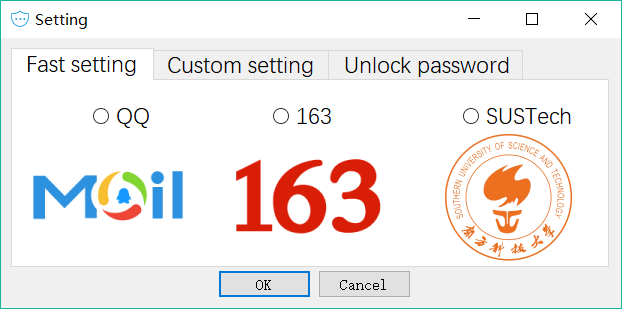
\includegraphics[width=0.5\textwidth]{UI3.png} 
			\caption{快速设置}
			\label{fig:Config_fast}
		\end{figure}
		\begin{figure}[H]
			\centering
			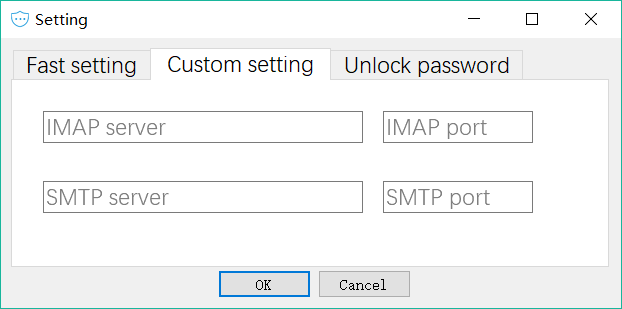
\includegraphics[width=0.5\textwidth]{UI4.png} 
			\caption{自定义设置}
			\label{fig:Config_custom}
		\end{figure}
		\begin{figure}[H]
			\centering
			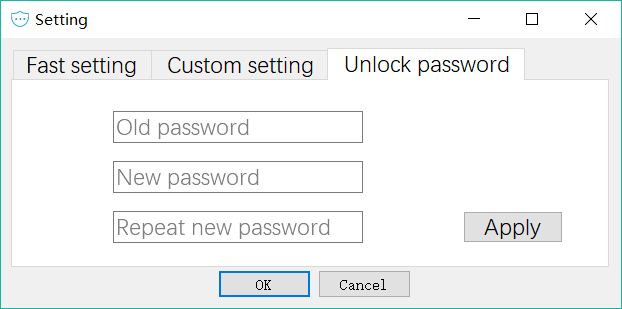
\includegraphics[width=0.5\textwidth]{UI5.png} 
			\caption{锁屏密码设置}
			\label{fig:Config_lockpwd}
		\end{figure}
	\end{enumerate}
	\item \textbf{聊天窗口}
	\\ 左侧栏目显示历史会话,右侧显示当前会话,输入框。
	\\ 历史会话右键可删除会话。
	\begin{enumerate}
		\item 发送图片、附件调用系统资源管理器获取待发送地址
		\item 添加联系人
		\item 创建群组,只能拉去自己的好友创建群组。
		\item 双击历史会话弹出群组详细信息窗户口,显示群组成员,右键可屏蔽成员。
	\end{enumerate}
	\item 非法操作提示窗口
	\\比如:输错密码时弹出。
	\item 锁屏密码输入窗口
	\\本地第二次登录时为了保护隐私需要输入锁屏密码。
\end{enumerate}

本次项目时间比较赶,项目逻辑代码实现就花了不少时间,留给各模块代码关联调试的时间不多。在项目开发的过程中,需要多沟通,时刻根据项目进度分配任务强度,确保按时完成项目。

\subsubsection{毛玉莲}
前期利用PGP加密协议,调用Python3 中的包gnupg和安装GPG软件生成了公钥和私钥,可以将公钥上传至MIT服务器,可以从服务器中取回对应公钥,但是因为生成的私钥无法转换成RSA格式,不能与王戈扬的文件加密解密部分对接,被舍弃。后期写了一半的报告。
	
	\begin{itemize}
		\item 生成密钥\\系统环境Ubuntu 16.04,可以通过GPG软件手动生成公钥和私钥,但无法通过Python 代码实现,非常令人费解的的是,我的代码在同学的电脑上可以生成公钥和私钥,在我的电脑上就不可以实现。
		最后发现,在我的电脑上需要设置绝对路径,默认路径无法使用,且通过命令行安装的gpg是1.4.0版本,需去官网
		下载手动安装2.2版本。
		\item 密钥格式转换\\ 王戈扬写好了对文件(消息和附件)加密解密的方法,但是使用的PEM格式的RSA算法,通过GPG生成的虽然也是PEM格式,但是不能直接将PEM格式的GPG密钥通过编码转换得到RSA类型的密钥。我后来在Github上找到了将公钥转换成RSA类型密钥的方法,但是找了很多资料也没有找到私钥转化的方法。
		\item 编码问题\\ gpg包不支持utf-8的编码,所以无法加密中文信息。
	\end{itemize}

通过这次的项目,我深刻认识到了合作的问题。一个项目,不是每一个人的部分做好了就可以了,最关键最难的地方在于与他人代码的拼接。在项目进行时,应该多一点交流而不是埋头只做自己的东西,导致做的部分与别人的脱轨。


\end{document}
